\section{Experimental results}
\label{section:results}
We have implemented the algorithms with multithreading supporting from
C++ 11 and conducted the experiments on Linux PCs with Intel Core i7
4790 processor with 4 cores, enabling 8 threads with the hyper
threading technology. We have used the Graph-cuts optimization code
written by Veksler, using the libraries provided by Boykov and
Kolmogorov~\cite{middlebury_mrf,alpha_expansion,what_energy_can_be_min_by_gc, mrf_experimental}.
% [2] Fast Approximate Energy Minimization via Graph Cuts.
%         Y. Boykov, O. Veksler, and R. Zabih.
%         In IEEE Transactions on Pattern Analysis and Machine Intelligence
%         (PAMI), vol. 23, no. 11, pages 1222-1239, November 2001.  
%
%     [3] What Energy Functions can be Minimized via Graph Cuts?
%         V. Kolmogorov and R. Zabih. 
%         In IEEE Transactions on Pattern Analysis and Machine Intelligence
%         (PAMI), vol. 26, no. 2, pages 147-159, February 2004. 
%         An earlier version appeared in European Conference on Computer
%         Vision (ECCV), May 2002.
%
%     [4] An Experimental Comparison of Min-Cut/Max-Flow Algorithms for
%         Energy Minimization in Vision. 
%         Y. Boykov and Vladimir Kolmogorov.
%         In IEEE Transactions on Pattern Analysis and Machine Intelligence
%         (PAMI), vol. 26, no. 9, pages 1124-1137, September 2004. 
We have used the QPBO and TRW-S implementations by
Kolmogorov~\cite{QPBO, TRW-S_implementation}.

\mysubsubsection{Stereo}

We performed our experiments on the Book sequence from Middlebury stereo
datasets.~\cite{middlebury_stereo}. We use 7 images with the
resolution of $695\times555$ and optimize for 256 disparity labels. We
recoreded both single thread energy and system energy (minimum energy
so far from all threads) against time. Since the order of labels to be
expanded or fused will have impact on minimization, we randomly
shuffled 256 labels and provide this order to all methods.

\begin{figure}[tb]
  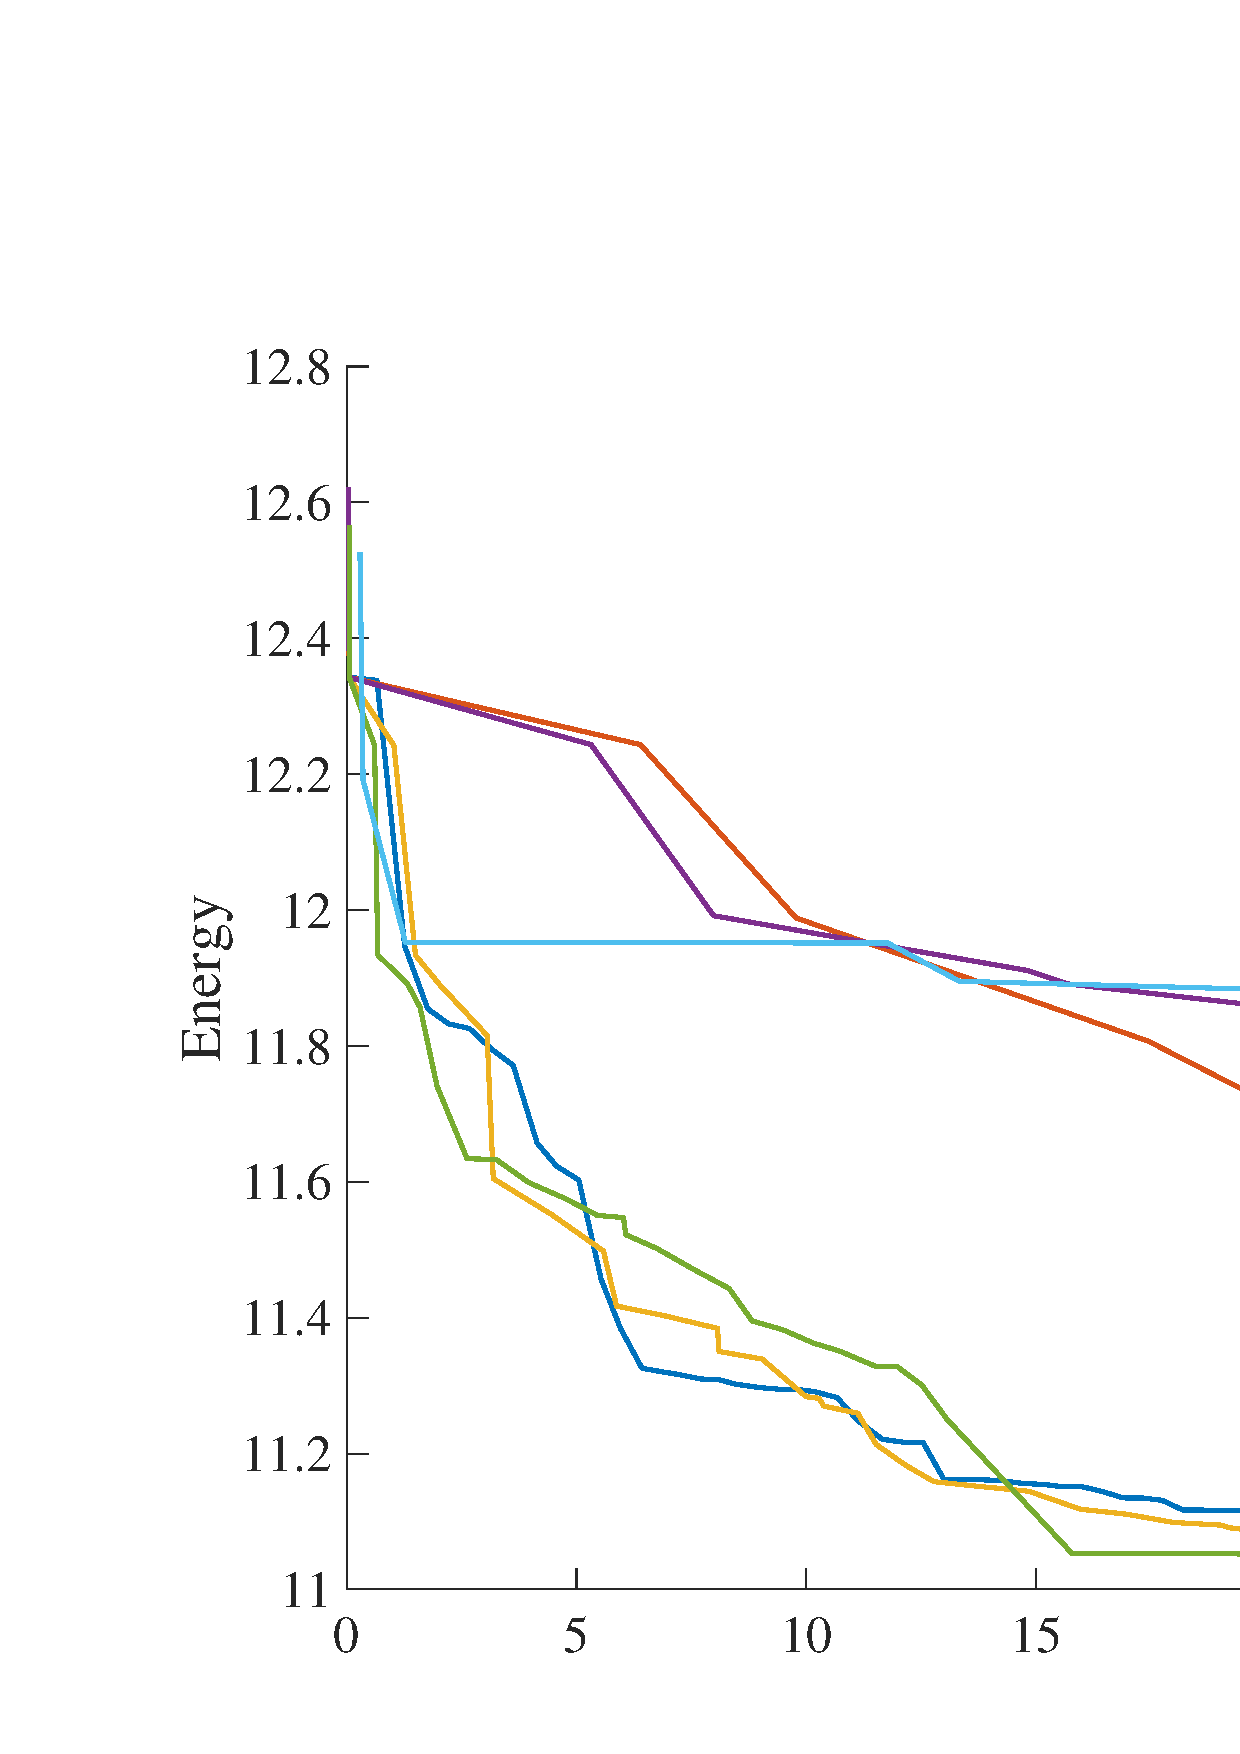
\includegraphics[width=\columnwidth]{figure/stereo_global.png}
  \caption{The energy minimization process of difference parallel systems.}
  \label{fig:stereo_global}
\end{figure}

\begin{figure}[tb]
  \includegraphics[width=\columnwidth]{figure/stereo_threads.png}
  \caption{Per thread energy. The left and right figures show the
    energy minimization process on each working thread of our method
    in SF-MF configuration and parallel $\alpha$-expansion method,
    respectively. The energy is in $\log$ scale}
  \label{fig:stereo_threads}
\end{figure}


Figure \ref{fig:stereo_global} shows the energy minimization process
against time. In this experiment, both PAE and SF-MF converge faster
than sequential method. However, since fusing solutions with multiple
labels by QPBO is slower than a single $\alpha$-expansion, PAE method
reaches convergence faster than SF-MF. Architectures with multiway
fusion, e.g. SF and SF-SS perform worse than PAE and SF-MF, because
the TRWS algorihtm used in multiway fusion is slower than multiple
$\alpha$-expansion. Finally, the line of hierarchy fusion only makes
jump when fusing on root node of the tree. This is because any fusion
step on non-root nodes only have partial label information.

Figure \ref{fig:stereo_threads} shows the per-thread energy
minimization process in SF-MF and PAE. The per-thread energy in SF-MF
architecture decreases more uniformly than that of PAE. In the
scenario where we need to query the best solution so far before the
whole optimization converges, SF-MF architecture is a better choice.

For a easy optimization problem as shown in this section, our full
architecture with solution sharing and multiway fusion actually makes
convergence slower by adopting sophisticated algorihtm and introducing
multi-threading overhead. However, we can easily configure the
architecture to make it better fit the problem, e.g. turn off multiway
fusion and/or solution sharing.



The figure illustrates the convergence rate of three competing methods
(alpha expansion, parallel alpha expansion, hierarchical fusion) against
our swarm fusion method.

%\hang{figure file missing}
\begin{figure}[tb]
  \includegraphics[width=\columnwidth]{figure/optical_flow_convergence.png}
  \caption{The energy minimization process for optical flow estimation of different methods. FS-MF has the best performance because of the solution sharing in early stage.}\label{fig:optical_flow_convergence}
\end{figure}
\begin{figure}[tb]
 \includegraphics[width=\columnwidth]{figure/layered_depthmap_convergence.png}
 \caption{The energy minimization process for layered depthmap estimation of different methods. Multi-way fusion is shown to be more effectvie than binary fusion in this problem setting.}\label{fig:layered_depthmap_convergence}
\end{figure}
\begin{figure}[tb]
  \includegraphics[width=\columnwidth]{figure/layered_depthmap_by_alpha.png}
  \caption{The energy minimization process for layered depthmap estimation with different $\alpha$ values. Multi-way fusion generally performs better than binary fusion, but the optimization becomes harder for using more ways in each step.}\label{fig:layered_depthmap_by_alpha}
\end{figure}
\begin{figure}[tb]
  \includegraphics[width=0.5\columnwidth]{figure/optical_flow_SF_MF_threads.png}
  \includegraphics[width=0.5\columnwidth]{figure/optical_flow_PFM_threads.png}
  \caption{Per thread energy. The left and right figures show the energy minimization process on each working thread of our method in SF-MF configuration and parallel fusion move, respectively.}\label{fig:optical_flow_by_threads}
\end{figure}
\begin{figure}[tb]
  \includegraphics[width=\columnwidth]{figure/optical_flow_by_beta.png}
  \caption{The energy minimization process for optical flow estimation with different $\beta$ values. Solution sharing generally makes energy minimization faster, but more solution sharing also means less time for exploring new solution proposals.}\label{fig:optical_flow_by_beta}
\end{figure}
\begin{figure}[tb]
  \includegraphics[width=\columnwidth]{figure/optical_flow_by_interval.png}
  \caption{The energy minimization process for optical flow estimation with different solution sharing frequency. Solution sharing generally makes energy minimization faster, but frequent solution sharing also means less time for exploring new solution proposals.}\label{fig:optical_flow_by_beta}\label{fig:optical_flow_by_interval}
\end{figure}


There are interesting pattern in the convergence plot of optical flow estimation problem. As both FS-MF and PAE are doing binary fusion, FS-MF finds lower energy faster than PAE. The reason is as follows. Some solution proposals are more effective than others, so once a thread grabs an effective solution proposal, it find a much lower energy. Since there is no solution sharing in PAE model, other threads cannot share this lower energy state, and keeps working on improving its own state. On the other hand, FS-MF allows solution sharing, so once a thread grabs an effective solution proposal and moves to a lower energy state, other threads can share this lower energy state. To further demonstrate what is happening here, we plot the energy-time for each thread in PAE and FS-MF in figure \ref{fig:optical_flow_by_threads}. As we can see from the plots, in PAE model, one thread finds lower energy state faster than others, while other threads keep working at their own energy state. But in FS-MF model, all threads exchange information about the lowest energy state and work on improving the lowest energy state together. So there are more chance of finding effective proposals faster and thus the energy goes down faster. Since the solution for optical flow can be locally improved by each thread, the final merging of PAE can effectively fuse good local results in different threads together and achieve a similar energy state with FS-MF model. Because FS-MF model shares information in the middle, a final merging becomes less necessary. Same comparison holds for FS-SS and FS.

To further understand the effect of solution sharing, we did two other experiments. In one experiment, we change the number of solutions each thread grabed from others from 0 to 3 (as there are 4 threads in total) while keeping others the same. The energy-time plots are shown in figure \ref{fig:optical_flow_by_beta}. As shown in the figure, energy decreases faster with solution sharing. While since we need to perform one fusion for sharing each solution, sharing more solution leads to unnecessary overhead in this problem setting. While sharing multiple solutions might be benefitial in some problem setting as it means each thread can get more global information early. In another experiment, we change the number of iterations between two consecutive solution sharing iterations as in figure \ref{fig:optical_flow_by_interval}. From the figure, we can see that although solution sharing generally speed up the optimization process, sharing solution too frequently is not a good practice. This is because When we share solution frequently, we have less time for generating and fusing new proposals. A good choice of the solution sharing frequency depends on specific problem setting.

From the convergence plot of layered depth map estimation, we can see that, Fusion Move, Parallel Fusion Move, and FS-MF all stalk at a high energy state. The reason is binary fusion of solution proposals (either from others or self) is too limited to further decrease the energy due to the complexity of the problem itself. Only when multi-way fusion is used (in FS-SS and FS), it becomes possible for the energy to further decrease. This coincides with the observation in \cite{layered_depthmap} that binary fusion of proposal solutions is not as powerful as their subspace fusion which is a special form of multi-way fusion here. To further explore the effect of multi-way fusion, we use different $\alpha$ {1, 3, 7, 15} in FS model while keeping other parameters the same and plot the energy-time curve in figure \ref{fig:layered_depth_map_by_alpha}.

As shown in \ref{section:results}, the multi-way fusion and solution sharing enabled by our uniform framework play a key role for improving performance in different settings. For better understanding our framework, we examine the role played by each factor more closely by varying each factor while keeping others the same.

